% !TEX TS-program = pdflatex
% !TEX encoding = UTF-8 Unicode

% This is a simple template for a LaTeX document using the "article" class.
% See "book", "report", "letter" for other types of document.

\documentclass[14pt]{article} % use larger type; default would be 10pt
\usepackage[14pt]{extsizes}
\usepackage[utf8]{inputenc} % set input encoding (not needed with XeLaTeX)
\usepackage[T2A]{fontenc}  %поддержка кириллицы в ЛаТеХ

\usepackage[titletoc]{appendix}
%%% Examples of Article customizations
% These packages are optional, depending whether you want the features they provide.
% See the LaTeX Companion or other references for full information.

%%% PAGE DIMENSIONS
\usepackage{geometry} % to change the page dimensions
\geometry{a4paper} % or letterpaper (US) or a5paper or....
\geometry{left=30mm, top=20mm, bottom=20mm, right=15mm} % for example, change the margins to 2 inches all round
% \geometry{landscape} % set up the page for landscape
%   read geometry.pdf for detailed page layout information

\usepackage[final]{graphicx} % support the \includegraphics command and options
\usepackage{epstopdf}
\let\bibsection\relax
\usepackage{amsmath}

%\usepackage[parfill]{parskip} % Activate to begin paragraphs with an empty line rather than an indent


%%% PACKAGES
\usepackage{amsfonts} %for \mathbb
\usepackage{amssymb}
\usepackage{dsfont}
\usepackage{booktabs} % for much better looking tables
\usepackage{array} % for better arrays (eg matrices) in maths
\usepackage{paralist} % very flexible & customisable lists (eg. enumerate/itemize, etc.)
\usepackage{verbatim} % adds environment for commenting out blocks of text & for better verbatim
\usepackage{subfig} % make it possible to include more than one captioned figure/table in a single float
\usepackage[english, russian]{babel}
\usepackage[hidelinks]{hyperref}
\usepackage{bookmark}
\usepackage{euscript}
\usepackage{caption}
\usepackage{pbox}
\usepackage[square,numbers]{natbib}
\setcitestyle{authoryear, open={[},close={]}}
% These packages are all incorporated in the memoir class to one degree or another...
%\usepackage{tempora}
\let\bibhang\relax
\let\citename\relax
\let\bibfont\relax
\let\Citeauthor\relax
\let\bibsection\relax
\expandafter\let\csname ver@natbib.sty\endcsname\relax
\usepackage[backend=bibtex,style=numeric]{biblatex}  %backend=biber is 'better'  

\addbibresource{kursach.bib}

\graphicspath{{img/}}

\usepackage{amsmath}
\usepackage{amstext}
%\usepackage{amssymb}
%\usepackage{bm}
%\usepackage{caption}
%\usepackage{color}
%\usepackage{epigraph}
%\usepackage{epsfig}
%\usepackage{float}
%\usepackage{gensymb}
%\usepackage{graphicx}
%\usepackage{hyperref}   
%\usepackage{mathtools}
%\usepackage{lipsum}
\usepackage{lscape}
\usepackage{setspace}
%\usepackage{indentfirst,latexsym}
%\usepackage{physics}
%\usepackage{setspace}
%\usepackage{subcaption}

%\onehalfspacing

\usepackage{xspace}

%%% HEADERS & FOOTERS
\usepackage{fancyhdr} % This should be set AFTER setting up the page geometry
\pagestyle{fancy} % options: empty , plain , fancy
\renewcommand{\headrulewidth}{0pt} % customise the layout...
\lhead{}\chead{}\rhead{}
\lfoot{}\cfoot{\thepage}\rfoot{}

%%% SECTION TITLE APPEARANCE
%\usepackage{sectsty}
%\allsectionsfont{\sffamily\mdseries\upshape} % (See the fntguide.pdf for font help)
% (This matches ConTeXt defaults)

%%% ToC (table of contents) APPEARANCE
\usepackage[nottoc,notlof,notlot]{tocbibind} % Put the bibliography in the ToC
\usepackage[titles,subfigure]{tocloft} % Alter the style of the Table of Contents
\renewcommand{\cftsecfont}{\rmfamily\mdseries\upshape}
\renewcommand{\cftsecpagefont}{\rmfamily\mdseries\upshape} % No bold!
\linespread{1.5}

\usepackage{indentfirst}

%%% END Article customizations



%\textheight 25.7cm % 29.7-2-2=25.7
%\textwidth 17cm % 21-2.5-1.5=17.0
%\hoffset -0.04cm %2.5-2.54=-0.04 слева 3см
%\voffset -1.04cm %2-2.54=0.54 сверху 2см
%\oddsidemargin 0cm
%\headheight 0cm
%\headsep 0cm
%\topmargin 0cm
%\setcounter{page}{1}
\def\sigspace{\\[1em]
\underline{\hspace{5cm}}\\[-0.2em]}

\usepackage{color,colortbl}

\definecolor{darkishgreen}{RGB}{39,203,22}
\definecolor{LightCyan}{rgb}{0.88,1,1}
\definecolor{Gray}{gray}{0.9}

\newcolumntype{g}{>{\columncolor{Gray}}c}
\newcolumntype{d}{>{\columncolor{darkishgreen}}c}


\begin{document}

\begin{titlepage}
	\begin{center}
		{
		{\bf Санкт-Петербургский Государственный Университет\\
		\vskip 1em
		Математико-механический факультет\\
		Кафедра Астрономии} }

	\vspace{3cm}
    	
	{\large А.С.\,Патшин}
    
    \vskip 2em
    

	\Large{\bf{Сравнение тригонометрических параллаксов звезд TGAS и Hipparcos}}
    \vskip 1em
    {\normalsize {Дипломная работа}\\}
	\end{center}
	
	\vskip 5em
    
	{
		 \begin{flushright}
			Научный руководитель:\\
		    доцент А.С.\,Цветков \sigspace
		    Рецензент:\\
		    PhD. З.М.\,Малкин \sigspace
		\end {flushright}
	}

	\vfill
	\begin{center}
	\small {Санкт-Петербург

	2018}
	\end{center}
\end{titlepage}

\newpage
\begin{titlepage}
	\begin{center}
		{
		{\bf Saint-Petersburg State University\\
		\vskip 1em
		Mathematics and Mechanics Department\\
		Chair of Astronomy} }

	\vspace{3cm}
    	
	{\large Anton Patshin}
    
    \vskip 2em
    

	\Large{\bf{Comparison of trigonometric parallaxes of TGAS and Hipparcos stars}}
    \vskip 1em

    {\normalsize {Graduation Thesis}\\}
	\end{center}
	
	\vskip 5em
    
	{
		 \begin{flushright}
			Scientific supervisor:\\
		    associate professor Alexander Tsvetkov \sigspace
		    Reviewer:\\
		    PhD. Zinovy Malkin \sigspace
		    
		\end {flushright}
	}

	\vfill
	\begin{center}
	\small {Saint-Petersburg

	2018}	
\end{center}
\end{titlepage}
\newpage
\tableofcontents
\newpage



 
\section{Введение}\label{introduction}

(Переписать этот пример под мою работу)


Сравнение каталогов является класической задачей фундаментальной\\ астрометрии, производщей переход от отдной системы координат к другой, оценить уровень систематических ошибок. До недавненго времени могло проводиться сравнение лишь положений и собственных движений.Появление первых результатов миссии GAIA, в частности, каталога TGAS, позволило впервые проихвести сравение тригонометрических параллаксов общих звезд каталогов TGAS и  Hipparcos, а именно его второй версии XHIP (XHIP: An extended hipparcos compilation, Anderson, 2012). Каталог TGAS содержит 2057050 звезд с данными о тригонометрических параллаксах, включает в себя только звезды Hipparcos и Tycho-2  и не является в полном смысле независимым продуктом, т.к. использует в качестве первой эпохи данные этих двух каталогов. Для сравнения мы используем общие звезды XHIP  и TGAS, которых оказалось 93635,из 117954 ожидаемых. из которыз пригодно для анализа 90283.

\subsection{Общие сведения о Hipparcos}\label{sub:smthhip}
 Тут мой супер классный диплом
$https://www.cosmos.esa.int/web/hipparcos/catalogue-summary$
$http://www.astronet.ru/db/msg/1210304/node2.html$

\subsection{Общие сведения о GAIA и TGAS}\label{sub:smthgaia}
Каталог GAIA

\section{Визуализация}\label{errvid}

\subsection{Проекция Хаммера}\label{sub:smthrs}

Визуализируем распределение звезд по небесной сфере воспользовавшить координатами из каталога TGAS. 

Для визуализации используем проекцию Хаммера . Которая представляет из себя проекцию карты с равной площадью, описанноая Эрнестом Хаммером в 1892 году (пример проекции на рис.~\ref{img:hammtiss}). Использяю ту же внешнюю форму с соотношением сторон 2:1, что и проекция Мользейде, Хаммера предназначена для уменьшения искажений в областях внешнх меридиан, которые очень велики в Мольвейде. 

\begin{figure}[h!]
\center{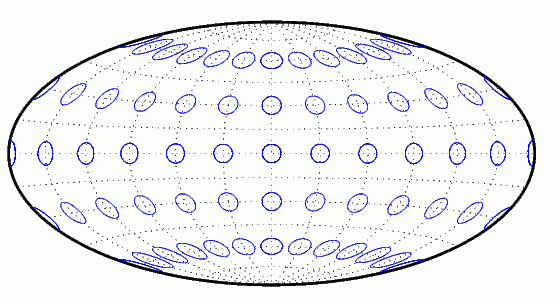
\includegraphics[width=0.7\linewidth]{hammtiss}}
\caption{Проекция Хаммера с сеткой и эллипсами равных площадей}
\label{img:hammtiss}
\end{figure}

Формулы преобразования на проекцию из сферической СК:
\begin{equation*}
\begin{array}{cl}
x = &\frac{2 \sqrt 2 \cos \varphi \sin \frac{\lambda}{2}}{\sqrt{1 + \cos \varphi \cos \frac{\lambda}{2}}}\\
y = &\frac{\sqrt 2\sin \varphi}{\sqrt{1 + \cos \varphi \cos \frac{\lambda}{2}}}\\
\end{array}
\end{equation*}

Перехода обратно осуществляется с помощью вспомогательного члена $z$:
\begin{equation*}
\begin{array}{lll}
z \equiv & \sqrt{1 - \left(\tfrac14 x\right)^2 - \left(\tfrac12 y\right)^2}\\
\lambda = & 2 \arctan \frac{zx}{2\left(2z^2 - 1\right)}\\
\varphi = & \arcsin {zy}
\end{array}
\end{equation*}

\subsection{Карты неба}\label{sub:smthrs}

Изрисунков~\ref{img:all_ra},~\ref{img:alllv},~\ref{img:alllon}, мы замечаем, что распределение звезд имеет характерный рисунок концентраии звезд в плоскости галактического экватора. На рисунке \ref{img:hixpix500}, для большей наглядности представлена шкала плотности в колличестве звезд на одну точку.

\begin{figure}[h!]
\center{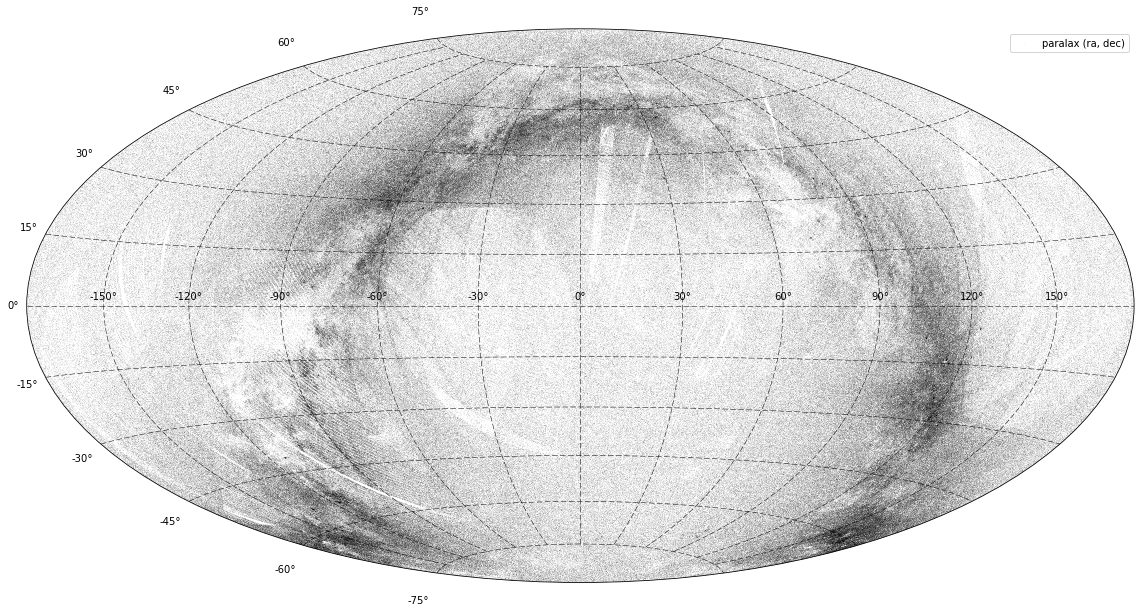
\includegraphics[width=0.7\linewidth]{all_ra}}
\caption{Распределение в экваториальной СК}
\label{img:all_ra}
\end{figure}
\begin{figure}[h!]
\center{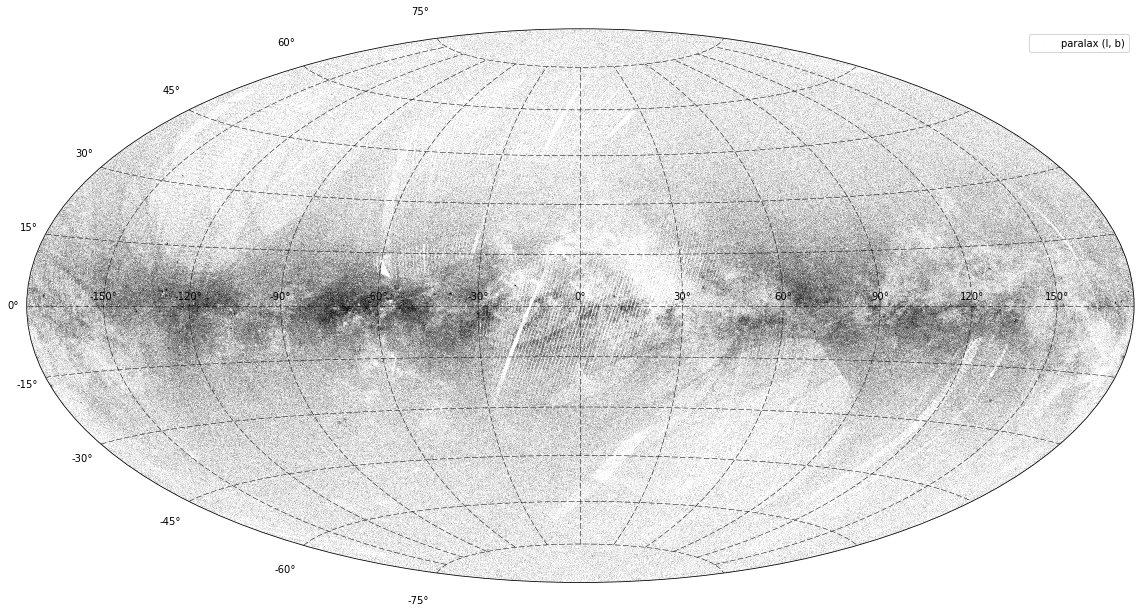
\includegraphics[width=0.7\linewidth]{alllv}}
\caption{Распределение в галлактической СК}
\label{img:alllv}
\end{figure}
\begin{figure}[h!]
\center{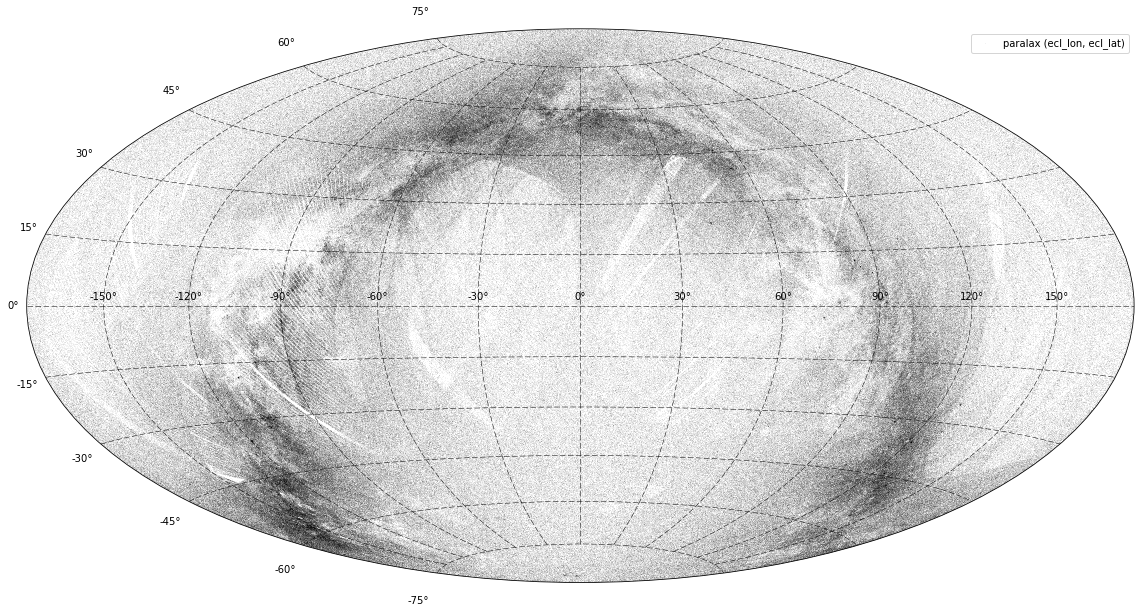
\includegraphics[width=0.7\linewidth]{alllon}}
\caption{Распределение в эклиптической СК}
\label{img:alllon}
\end{figure}
\begin{figure}[h!]
\center{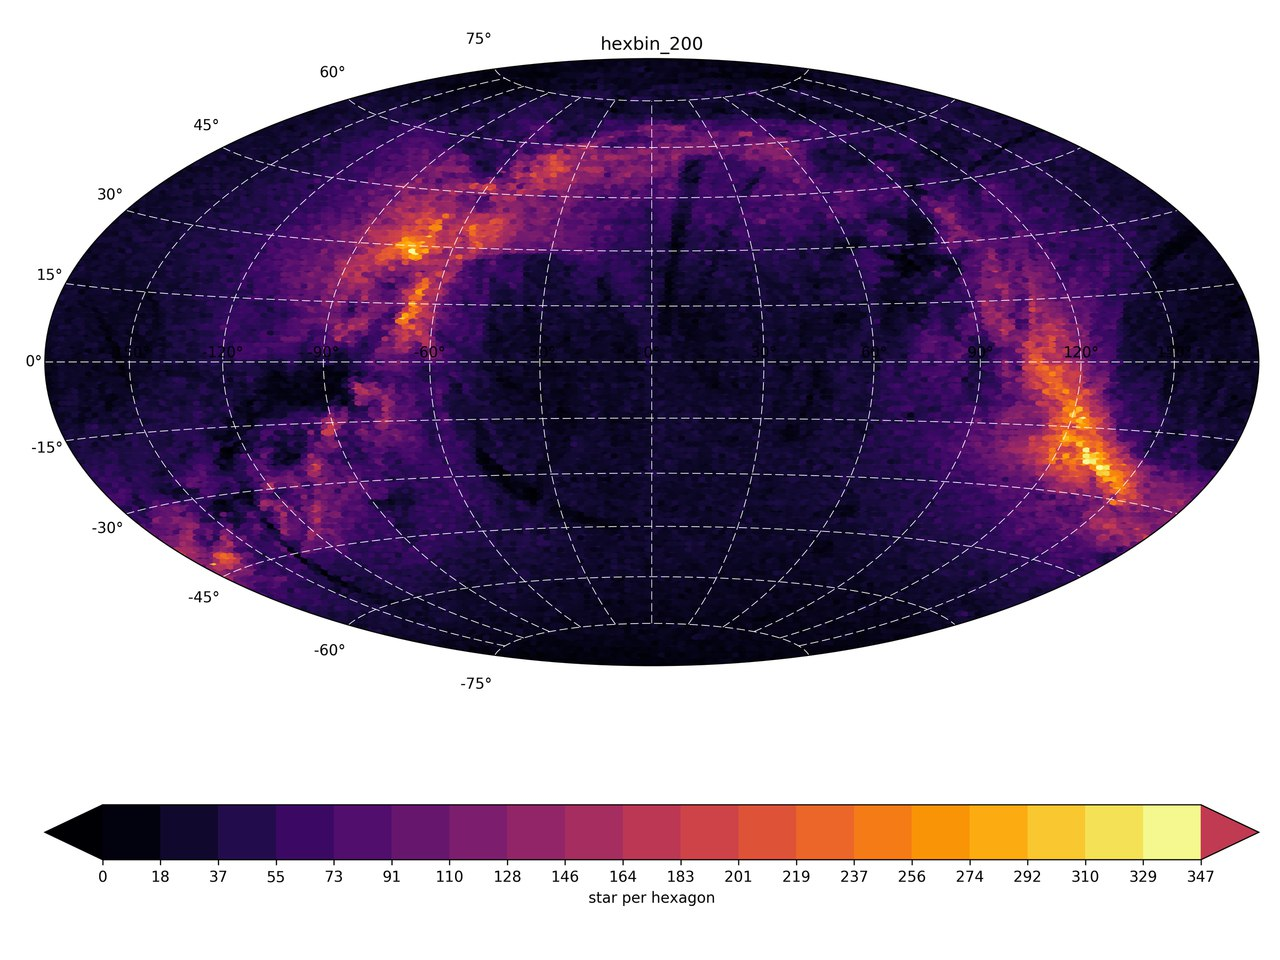
\includegraphics[width=0.7\linewidth]{hixpix500}}
\caption{Распределение численности звезд, в экваториальной СК}
\label{img:hixpix500}
\end{figure}

\subsection{Выборка данных}\label{sub:smthzd}
У каждой звезд в каталоге TGAS есть идентификатор из каталога Hipparcos, объеденим данные двух каталогов для каждой звезды. Таким образом в объединённом каталоге будут данные из каталога XHIP и TGAS. В каталоге XHIP 117955 объектов. В TGAS -- 2057050. В их объединении -- 93635, Из котрых, пригодны для качественного сравнения тригонометрических параллаксов -- 90283 ($\pi_{hip} > 0$ и $\pi_{tgas}>0$).


Интересующие нас поля из каталога XHIP:

\begin{itemize}

\item $id$ - идентификатор звезды в каталоге Hipparcos

\item $\pi_{xhip}$ - абсолютный барицентрический параллакс звезды на момент эпохи каталога, указано в mas

\item $\delta_{\pi_{xhip}}$ - стандартное отклонение параллаксов звезды на момент эпохи каталога, указано в mas

\item $n_{obs}$ - количество наблюдейний данной звезды аппаратом Hipparcos

\end{itemize}

Из каталога TGAS нас интересуют следующие поля

\begin{itemize}

\item $hip$ - идентификатор звезды в каталоге Hipparcos

\item $\pi_{tgas}$ - абсолютный барицентрический параллакс звезды на момент эпохи каталога, указано в mas

\item $\delta_{\pi_{tgas}}$ - стандартное отклонение параллаксов звезды на момент эпохи каталога, указано в mas

\item $ra$ - экваториальная долгота на момент эпохи каталога, указано в градусах

\item $dec$ - экваториальная широта на момент эпохи каталога, указано в градусах

\item $l$ - галактическая долгота на момент эпохи каталога, указано в градусах

\item $b$ - галактическая широта на момент эпохи каталога, указано в градусах

\item $lon$ - эклиптическая долгота на момент эпохи каталога, указано в градусах

\item $lat$ - эклипическая широта на момент эпохи каталога, указано в градусах

\end{itemize}

\section{Построение и предварительный анализ}\label{errvid}
<Переписать>
Астрометрические каталоги всегда сравнивали между собой, для выявления случайных иособенно важных, систематических ошибок. Благодаря каталогам TGAS и XHIP, имеется возмодность произвести сравнение параллаксов, полученных тригонометрическим способом для столько большого колличества объектов. К сожалению, параллаксы XHIP и TGAS  не являются независимыми величинами. Корректную процедура сравнения возможно лишь после выхода второй, а то и большей редакции каталога~\cite{wiki:gaia}, где параллаксы будут получены независимо от данных аппарата Hipparcos.

РАссмотрим для каждой звезды общего каталога величину разности параллаксов в XHIP и в TGAS, т.е. $\pi_{xhip} - \pi_{tgas}$. Ошибкой разности, соответственно, будем считать $\sqrt{\delta^2_{\pi_{xhip}} + \delta^2_{\pi_{tgas}}}$. Для начала выпишем различные статистические характеристики данной величины. СРеднее значение - 0.35 mas, Медиана 0.29, Стандартное отклонение -- 1.5 mas, Среднее значение модуля -- 1.04 mas, Медиана модуля - 0.76 mas, 99 персентиль модуля - 4.78 mas. 

Обычно систематические разности положений и собственных движений изучают в эквивалентной, в силу зонного построения каталогов, или галактической системе для массивных звездных каталогов, в котрых распределение звезд в этой системе симметрично (ссылка на работы витязева и цветкова?). Первое знакомство с систематическими разностями параллаксов (пир 4) показывает, что присутствует симметрия разностей относительно эклиптики.

Более того, мы видим зависимость между модулем разности параллаксов на рис.4 и ошибкой параллаксов в XHIP на рис.6  в эклиптической системе координат. Действительно, коэффицент корреляции между этими величинами на звездах объего каталога равен 0.55. Это говорит о том, что чем выше ошибка параллакса XHIP, тем сильнее он отличается от параллакса TGAS.

\section{Анализ больших выборосов}\label{errvid}
Рассмотрим звезды у которых параллаксы в XHIP и TGAS  значимо различаются, а именно, у которых модуль разности параллаксов больше, чем 3 ошибки этой разности. Таких звезд 2148. Выясним, с чем связаны такие отличия в параллаксах. У таких звезд коэффициент корреляции моуля разности параллаксов с ошибкой параллакса в XHIP равен 0.87, а с ошибкой в TGAS -- 0.1. Т.е. можно утверждать. что большая разница медлу параллаксами обусловленна большими ошибками параллаксов именно в XHIP/ Явно ошибочными являются параллаксы меньше 0, т.е. это такие паралаксы $\pi$ , что $\pi < -3\delta_{\pi}$. В TGAS таких звезд всего 6, а в XHIP - 17. Т.е. подобного рода выбросы не должны сильно влиять на усредненные характеристики разности параллаксов XHIP и TGAS.





\subsection{случайные выбросы}\label{sub:smthrs}



\section{Анализ разностей с помощью сферических функций}\label{sistem}
 На рис.4 мы видим явную зависимость в распределении модуля отличия параллаксов по небесной сфере от модуля эклиптической широты (коэффициент корреляции равен -0.7).  Подтвердить статистическую значимость данной зависимости и незначимость прочих менее очевидных зависимостей мы можем с помощью представления модуля разностей параллаксов через сферические функции. Сферические функции широко используются в различных областях математики и физики, их определение можно найти во многих источниках (см., например, Арфкен, 1970). Впервые  были использованы для анализа систематических разностей положений и собственных движений (броше 1977). Мы впервые используем этот инструмент для анализа систематических разностей параллаксов.
 
Представление модуля разницы параллаксов с помощью линейной комбинации сферических функций можно записать следующим образом.


$$ \Delta_{plx} (l,b) = \sum_{nkp}\delta_{nkp}K_{nkp}(l,b) $$,
где сферические функции имеют вид (Арфкен, 1970)~\cite{book:arfken}.

\begin{equation}\label{f:sf_k}
K_{nkp}(l,b) = R_{nk} \left\{ \begin{array}{ll}
P_{n,0}(b), & \textrm{$k=0, p=1$,}\\
P_{n,k}(b)\sin{kl}, & \textrm{$k\neq0, p=0$,}\\
P_{n,k}(b)\cos{kl}, & \textrm{$k\neq0, p=1$,}
\end{array} \right.
\end{equation}

\begin{equation}
R_{nk} = \sqrt[]{\frac{2n+1}{4\pi}} \left\{ \begin{array}{cc}
\sqrt[]{\frac{2(n-k)!}{(n+k)!}}, & \textrm{$k>0$,}\\
1, & \textrm{$k=0$,}
\end{array} \right.
\end{equation}

В формуле (\ref{f:sf_k}) через $l$ и $b$ обозначены соответственно долгота и широта на сфере, ($0 \leq l \leq 2\pi$; $-\pi/2\leq b \leq \pi/2$); через $P_{nk}(b)$ - полиномы лежандра (при $k = 0$) и присоединенные функции Лежандра (при $k > 0$), которые можно вычислить с помощью следующих рекуррентных соотношений. 
\begin{equation}
\begin{array}{rll}
P_{nk}(b)=&\sin{b\frac{2n-1}{n-k}}P_{n-1,k}(b)-\frac{n+k-1}{n-k}P_{n-2,k}(b), & {}^{k=0,1,...}_{n=k+1,k+2,...}\\
P_{kk}(b)=&\frac{(2k)!}{2^{k}k!}{\cos{b}}^{k}\\
P_{k+1,k}(b)=&\frac{(2k+2)!}{2^{k+1}(k+1)!}{\cos{b}}^{k}\sin{b}
\end{array}
\end{equation}

Для практичности часто вводят линейную нумерацию  сферических коэффициентов $\beta_{nkp}$ и функций $K_{nkp}$ c помощью одного индекса $j$, где

\begin{equation}\label{f:sf_j}
j = n^2 + 2k + p -1
\end{equation}

Каждый может убедиться, что введёные сферические функции удовлетвояют следующим соотношениям:

\begin{equation}
\iint\limits_\Omega \left(K_i \cdot K_j \right) d\omega =  \left\{ \begin{array}{cc}
0, & i \neq j,\\
1, & i = j.
\end{array} \right.
\end{equation}

bИными словами, набор функций $K_{nkp}$ образует на сфере ортонормированную систему функций.






\section{Систематические различия}\label{sistem}
		

\subsection{Healpix}\label{sub:smthhealpix}
HEALPix -- это абревиатура \textbf{H}ierarchical \textbf{E}qual \textbf{A}rea iso\textbf{L}atitude \textbf{Pix}elation of a sphere (Иерархическая равная изоляционная площадь пикселей). 

Первоначальным мотивом для разработки HEALPix была мпутниковая миссия NASA (http://map.gsfc.nasa.gov/) сана по измерению <>, и в настоящее время действует миссия ESA Planck -- созданию полномасштабной карты реликтового излучения (микроволного анизотропного поля) с угловым разрешением несколько угловых секунд. Основными требования при разработке HEALPix, было создание математической структуры, которая поддерживает подходящую дискретизацию функций на сфере при достаточно высоком разрешении и облегчает быстрый и точный статистический и астрофизический анализ массивных наборов данных полного неба.

HEALPix удовлетворяет этим требованиям, поскольку обладает следующими тремя существенными свойствами:

\begin{itemize}
\item Сфера иерархически тесселирована в криволинейный четырёхугольник. Проекция с самым низким разрешением состоит из 12 базовых пикселей. Разрешение тесселяции увеличивается за счёт деления каждого пикселя на четыре новых. На следуюзщем рисунке (\ref{img:healpix}) показано (по часовой стрелке от верхнего левого до нижнего левого)разрешение увеличивается на 3 шага от базового уровня (т.е. сфера разделена соответственнно на 12, 48, 19 и 768 пикселей).
\item Области/Площади всех пикселей при заданном разрешении идентичны.
\item Пиксели распределены по линиям постоянной широты. Это свойство необходимо для всех приложений гармонческого анализа с участием сферических гармоник. Из-за изо-широтного распределения точек выборки скорость вычисления интегралов по отдельным сферическким гармоникам масштабируется как $~N^{1/2}$ с общим колличеством пикселей, в отличае от пасштабирования $~N$ для распределений выборки неизото-широты(?) (примерами которой является четырёхгранный сферический куб ($http://lambda.gsfc.nasa.gov/product/cobe/skymap_info_new.cfm$), используемый для COBE ($http://lambda.gsfc.nasa.gov/product/cobe$) NASA данные и любое распределение, основанное на симметрии икосаэдра).
\end{itemize}

\begin{figure}[h!]
\center{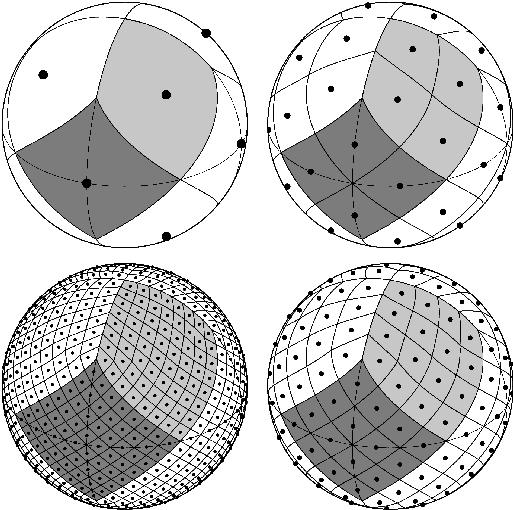
\includegraphics[width=0.5\linewidth]{healpix}}
\caption{Деление сферы на равные по пложади сигменты.}
\label{img:healpix}
\end{figure}

Другим свойством сетки HEALPix является то, что пиксельные центы, представленные черными точками, встречаются на конечном числе колец постоянной широты, количество колец зависит от разрешения сетки HEALPix. Для примера, у зеленогой, желтой, красной и синей сферы их 3, 7, 15, 31 кольцо с постоянной широтой соответственно(?).

Ниже, на рисунке~(\ref{img:cmb}) приведён пример применения HEALPix с высоким разрешением -- Модель реликтового излучения (CMB) (космическое сверхвысокочастотное фоновое излучение), состоящая из 12582912 пикселей (~ 3.4 минут дуги (arcmin)).


\begin{figure}[h]
\begin{minipage}[h]{0.3\linewidth}
\center{
\includegraphics[width=1\linewidth]{exampleCMB} \\На сфере}
\end{minipage}
\hfill
\begin{minipage}[h]{0.69\linewidth}
\center{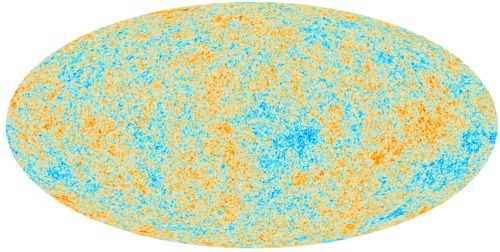
\includegraphics[width=0.85\linewidth]{Planck-CMB-map-at-high-resolution_planck_cmb_map} \\Проекция Hammer}
\end{minipage}
\caption{Визуализация CMB на HEALPix}
\label{img:cmb}
\end{figure}


HealPix имеет два режима разбиения:
\begin{itemize}
\item NEST - позволяет работать со сферическими функциями и не только...

\item RING - позволяет определять минимальное расстояние до точек и не только...
\end{itemize}

\begin{figure}[h]
\begin{minipage}[h]{0.48\linewidth}
\center{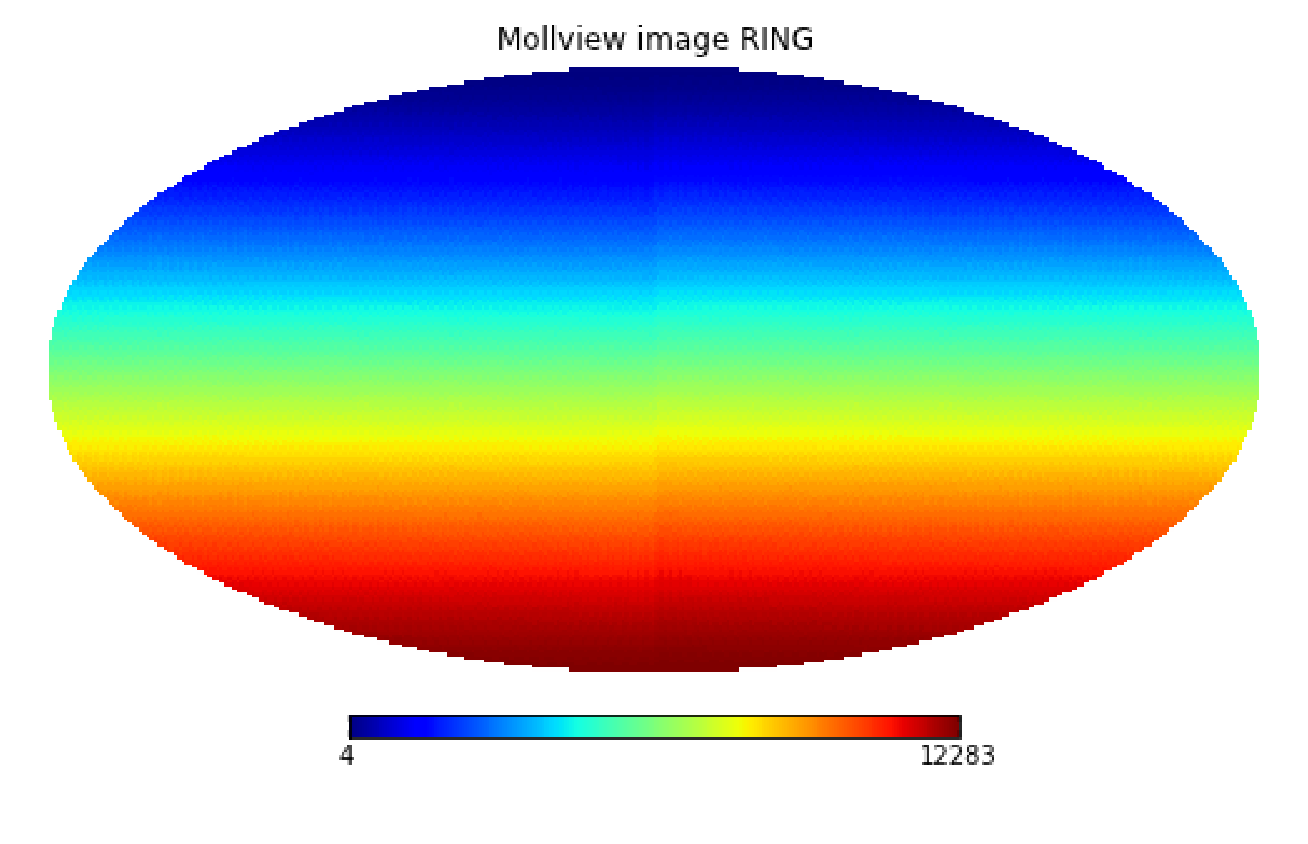
\includegraphics[width=1\linewidth]{moll_nside32_ring}}
\end{minipage}
\hfill
\begin{minipage}[h]{0.48\linewidth}
\center{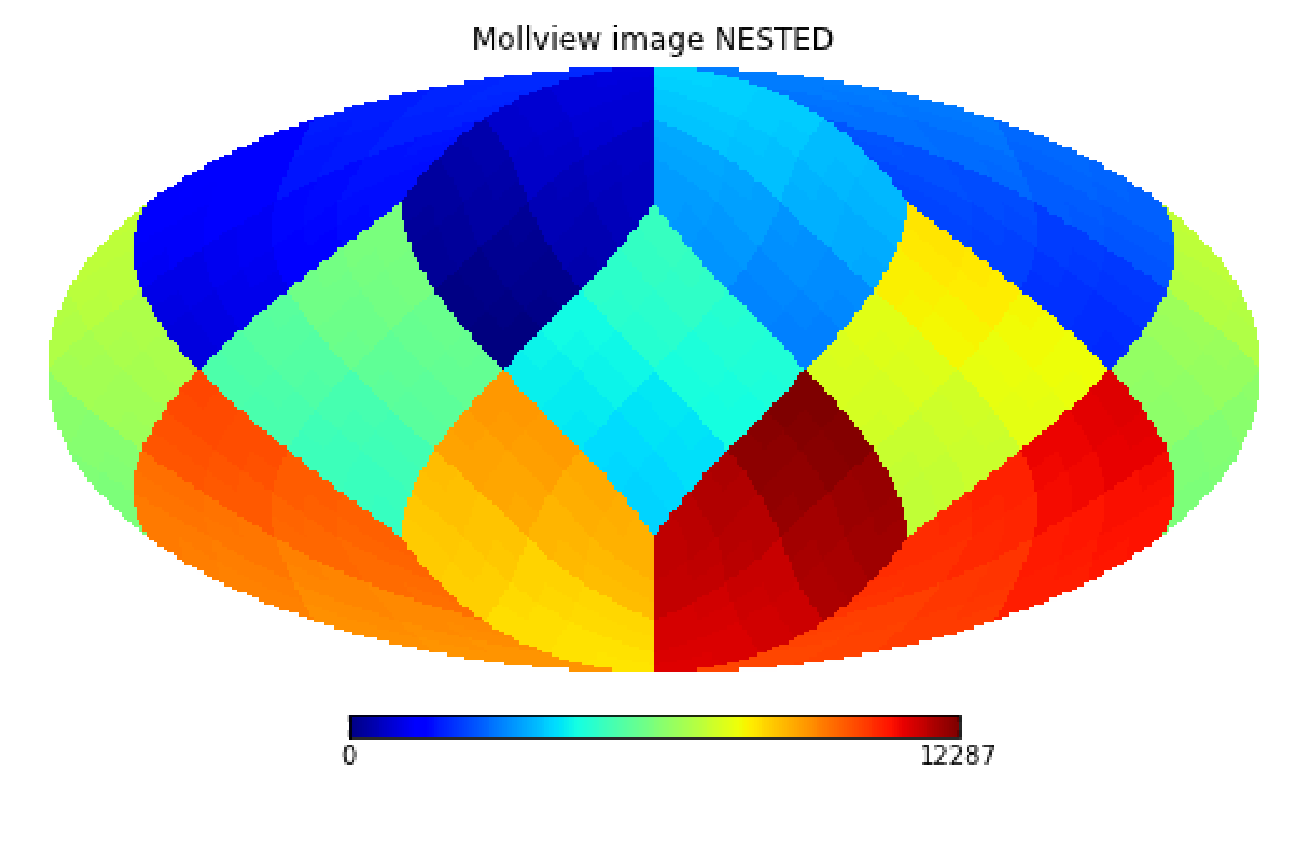
\includegraphics[width=1\linewidth]{moll_nside32_nest}}
\end{minipage}
\caption{Пример распределения  пикселей по ring and nest}
\label{ris:moll_nside32_healpix}
\end{figure}

Для нашей задачи отлично подходит NEST.

~\cite{wiki:healpix} 


Представление модуля разницы параллаксов с помощью линейной комбинации сферических функций.

$\delta_{plx}(l,b) = \sum_{nkp}\delta_{nkp}K_{nkp}(l,b)$



tgas
2026210 > 0
30840 < 0


\begin{table}[h!]
\centering
\caption{Общая статистика по параллаксам и их ошибкам в каталоге TGAS}
\label{tabular:tgas_st}
\begin{tabular}{c|c|c}
%\rowcolor{Gray} 
{}&parallax &parallax error\\
\hline 	
count &2057050	&2057050\\
mean	&2.477627e+00	&3.850052e-01\\
std	&2.910183e+00	&1.699272e-01\\
min	&-2.481995e+01	&2.039740e-01\\
25\%	&1.030510e+00	&2.681603e-01\\
50\%	&1.780198e+00	&3.220124e-01\\
75\%	&3.015706e+00	&4.360010e-01\\
max	&2.958036e+02	&9.999985e-01\\
\end{tabular}
\end{table}

dgh
%статистика за 75 максимальных паралаксов
$$ 
	hip	parallax	parallax_hip	parallax_difference	parallax_difference_abs	parallax_error	parallax_error_hip	nobs
count	75.000000	75.000000	75.000000	75.000000	75.000000	75.000000	75.000000	75.00000
mean	56748.066667	10.741791	32.820133	22.078342	26.850197	0.361560	11.996400	108.60000
std	35019.201714	19.991696	18.491322	19.794312	12.457118	0.161835	6.597439	47.07527
min	570.000000	0.325257	1.620000	-42.350255	15.379289	0.228392	1.210000	41.00000
25%	26286.500000	1.872400	21.840000	17.414510	18.460047	0.262694	8.125000	78.00000
50%	58241.000000	4.355962	30.020000	22.802842	24.085758	0.303822	11.610000	95.00000
75%	90761.000000	9.636104	40.240000	30.286968	30.684965	0.379440	14.930000	133.00000
max	117081.000000	148.510255	106.160000	90.056481	90.056481	0.941835	47.480000	266.00000
$$

$$
	parallax_hip	parallax_error_hip	nobs
count	117955.000000	117955.000000	117955.000000
mean	7.210770	1.118005	115.967750
std	11.492073	1.668194	42.755056
min	-258.450000	0.090000	20.000000
25%	2.530000	0.660000	85.000000
50%	4.610000	0.900000	111.000000
75%	8.430000	1.230000	139.000000
max	796.920000	259.410000	388.000000
tgas + hip
	parallax	parallax_error	parallax_hip	parallax_error_hip	parallax_difference	parallax_difference_abs	parallax_error_hip_tgas
count	93635.000000	93635.000000	93635.000000	93635.000000	90283.000000	9.028300e+04	93635.000000
mean	6.619395	0.331578	6.716317	1.098058	0.213103	1.071412e+00	1.167708
std	8.475341	0.136050	8.682223	0.982716	1.712709	1.353089e+00	0.967663
min	-23.702470	0.203974	-118.140000	0.090000	-42.350255	5.408112e-07	0.330823
25%	2.375351	0.246761	2.470000	0.690000	-0.614582	3.560939e-01	0.773412
50%	4.205981	0.283109	4.490000	0.920000	0.140436	7.788567e-01	0.991394
75%	7.789418	0.357870	8.110000	1.230000	0.934272	1.406570e+00	1.290527
max	295.803638	0.999889	298.040000	47.480000	90.056481	9.005648e+01	47.481203
t	parallax_hip	parallax_error_hip	nobs
count	93635.000000	93635.000000	93635.000000
mean	6.716317	1.098058	117.493384
std	8.682223	0.982716	42.979748
min	-118.140000	0.090000	20.000000
25%	2.470000	0.690000	86.000000
50%	4.490000	0.920000	113.000000
75%	8.110000	1.230000	140.000000
max	298.040000	47.480000	388.000000
$$


\section{Заключение}\label{conclusion}
В ходе решения задач было разработано программное обеспечение для работы с каталогом TGAS и XHIP, визуализации данных и разложения на сферические гармоники. Были получены коэффициенты разложения в сферические функции для различных раборов данных в разных Небесных сферах. (Раздел 4.2).
Данная работа носит подготовительный характер для обработки последующих релизов каталога Gaia, в том числе релиза Gaia
Data Release 2, вышедшего 25 апреля 2018 года. В новой версии каталога значитель-но увеличилось число объектов, для которых известны пять астрометри-ческих параметров.

\newpage
\section{Список использованной литературы}\label{conclusionlit}
%\bibliographystyle{unsrt}
%\bibliography{kursach.bib}
\printbibliography[type=online,title={Online only}]
\printbibliography[type=book,title={Статьи:}]


\appendix

\section*{Приложение}
тут аппендикс или два 

\newpage
\begin{landscape}
\begin{spacing}{1.0}
%\rotatebox{90}{ %это обеспечивает поворот любого объекта
%\begin{minipage}{1.6\linewidth}
\begin{table}[h]
\caption{Рекордсмены по разности параллаксов}
\label{tabular:75_25}
\begin{tabular}{|r|r|r|r|r|r|r|r|}
\hline 	
$hip_{id}$ &$\pi_{tgas}$ &$\pi_{hip}$ &$\pi_{difference}$ &$\pi_{difference_{abs}}$ &$\pi_{error_{tgas}}$ &$\pi_{error_{hip}}$ &$n_{obs_{hip}}$\\
\hline 
21000&3.6135194843037333&93.67&90.05648051569626&90.05648051569626&0.43092538640597655&7.62&41\\
42525&5.939340804931861&68.54&62.60065919506815&62.60065919506815&0.4989712380569283&15.51&88\\
117081&7.767833345528349&63.56&55.79216665447166&55.79216665447166&0.391415724958141&21.02&52\\
92059&1.0253014604321609&55.49&54.46469853956784&54.46469853956784&0.2575126107035069&13.48&74\\
16582&3.3525394898163663&46.79&43.43746051018363&43.43746051018363&0.3379833330672927&47.48&78\\
49971&10.032882741927454&53.21&43.17711725807255&43.17711725807255&0.2739555697690759&17.78&79\\
14101&148.51025482141657&106.16&-42.35025482141657&42.35025482141657&0.9418350466246392&16.51&95\\
90368&9.239325596436997&51.0&41.760674403563&41.760674403563&0.2380419233789036&10.37&128\\
87784&0.9016399080820414&41.3&40.398360091917965&40.398360091917965&0.2617397591615193&8.36&266\\
11167&1.6005219496065075&40.32&38.71947805039349&38.71947805039349&0.36195791278945777&18.63&146\\
17468&3.6968394746639017&41.4&37.703160525336095&37.703160525336095&0.9324727968205918&15.72&62\\
26690&6.758462929784543&43.01&36.251537070215456&36.251537070215456&0.2790695120679915&28.39&55\\
63028&6.593468516719788&41.33&34.73653148328021&34.73653148328021&0.38054460916425065&10.0&140\\
2715&8.99457132952772&43.6&34.605428670472286&34.605428670472286&0.36759122490605495&15.16&73\\
43650&1.8692458424123573&36.4&34.530754157587644&34.530754157587644&0.2636490611144113&8.77&131\\
37103&1.177487047842296&33.63&32.452512952157704&32.452512952157704&0.23851513809910355&20.31&52\\
8356&1.875554375591414&33.99&32.11444562440859&32.11444562440859&0.3490448951334293&20.35&89\\
33404&1.6814129603685233&33.48&31.798587039631478&31.798587039631478&0.2728863787154474&16.3&261\\
35873&1.7659760403953777&32.58&30.814023959604626&30.814023959604626&0.3144475734924109&11.18&84\\
109335&3.5040942969592948&34.06&30.55590570304071&30.55590570304071&0.2418385213119765&8.86&123\\
109930&2.941969216919245&32.96&30.018030783080764&30.018030783080764&0.23828269976331&12.73&127\\
26111&0.8614923854606678&30.22&29.358507614539327&29.358507614539327&0.2734412733226204&1.94&247\\
99720&6.2138396569790295&35.41&29.196160343020967&29.196160343020967&0.4081948331799583&9.14&84\\
26462&7.749974783835219&36.88&29.130025216164785&29.130025216164785&0.2542881333731009&15.57&94\\
86685&2.5910519158726935&30.58&27.98894808412731&27.98894808412731&0.22941196532598346&14.02&62\\
\hline 
\end{tabular}
\end{table}

\newpage

\begin{table}[h]
\caption{Рекордсмены по разности параллаксов}
\label{tabular:75_50}
\begin{tabular}{|r|r|r|r|r|r|r|r|}
\hline 	
$hip_{id}$ &$\pi_{tgas}$ &$\pi_{hip}$ &$\pi_{difference}$ &$\pi_{difference_{abs}}$ &$\pi_{error_{tgas}}$ &$\pi_{error_{hip}}$ &$n_{obs_{hip}}$\\
\hline 
101453&0.47229964249774603&27.73&27.25770035750225&27.25770035750225&0.3815522125350718&22.97&72\\
80365&0.3252566015932853&27.29&26.964743398406714&26.964743398406714&0.2991317461151089&17.1&105\\
570&2.286728392538792&28.95&26.66327160746121&26.66327160746121&0.29479727936398475&12.23&116\\
66125&29.328255835837076&55.78&26.45174416416293&26.45174416416293&0.28838700860065314&10.02&142\\
91557&56.48334976858664&30.49&-25.993349768586643&25.993349768586643&0.26665022041629555&7.89&71\\
100625&2.6086537349321026&27.99&25.381346265067897&25.381346265067897&0.4762157223925944&7.06&88\\
111276&4.355962433196507&29.73&25.374037566803487&25.374037566803487&0.2491454760570632&7.24&106\\
47645&31.714569962446753&6.92&-24.79456996244675&24.79456996244675&0.5027812716747218&4.05&97\\
47846&2.0769676160399926&26.74&24.663032383960005&24.663032383960005&0.3718433605661264&13.43&119\\
96643&6.704986888643228&31.35&24.645013111356768&24.645013111356768&0.6719925058062542&10.99&86\\
64289&5.528102793567756&30.02&24.491897206432238&24.491897206432238&0.2729570135141233&12.06&216\\
46637&28.667826266554712&52.99&24.322173733445286&24.322173733445286&0.3057977692475484&13.11&62\\
14137&15.784241966318724&39.87&24.085758033681273&24.085758033681273&0.9159903829184022&10.61&114\\
31998&1.4152700481213487&24.89&23.474729951878647&23.474729951878647&0.3038217166099563&8.85&105\\
74143&4.583228557144263&27.83&23.24677144285573&23.24677144285573&0.2362874545789483&14.7&53\\
47839&17.35715805587964&40.16&22.80284194412036&22.80284194412036&0.2874781695636456&7.14&143\\
7739&0.5226712293088758&22.68&22.157328770691123&22.157328770691123&0.4886794246222954&11.61&139\\
7197&5.962195894692861&27.71&21.74780410530714&21.74780410530714&0.2822776116397612&7.8&152\\
68158&1.0248438291894155&22.71&21.685156170810586&21.685156170810586&0.25628523607246856&9.75&93\\
5669&5.099146141909381&25.94&20.840853858090615&20.840853858090615&0.5073643719931885&15.48&56\\
70446&10.257532551168296&30.89&20.632467448831704&20.632467448831704&0.2638598628788957&10.84&140\\
91154&26.083310925789466&46.71&20.62668907421053&20.62668907421053&0.7623642510543536&1.44&80\\
95652&5.5940400684495994&25.56&19.965959931550397&19.965959931550397&0.3290609310114135&13.67&113\\
93722&0.44814565033275344&20.39&19.941854349667246&19.941854349667246&0.29492235794973065&10.76&122\\
58241&28.22518406478849&8.35&-19.87518406478849&19.87518406478849&0.2582119869663121&10.74&86\\
\hline 
\end{tabular}
\end{table}

\newpage

\begin{table}[h]
\caption{Рекордсмены по разности параллаксов}
\label{tabular:75_75}
\begin{tabular}{|r|r|r|r|r|r|r|r|}
\hline 	
$hip_{id}$ &$\pi_{tgas}$ &$\pi_{hip}$ &$\pi_{difference}$ &$\pi_{difference_{abs}}$ &$\pi_{error_{tgas}}$ &$\pi_{error_{hip}}$ &$n_{obs_{hip}}$\\
\hline 
10332&0.5496683653487973&20.29&19.7403316346512&19.7403316346512&0.34515024281556256&9.42&118\\
41955&7.370182159796287&26.92&19.549817840203715&19.549817840203715&0.2421192538511551&5.33&149\\
58988&0.8162321311506745&19.89&19.073767868849327&19.073767868849327&0.3197442591937322&12.5&140\\
42652&3.256530578152378&22.11&18.85346942184762&18.85346942184762&0.2298275358550482&5.91&189\\
75262&4.753556800163254&23.58&18.826443199836746&18.826443199836746&0.2326450723449282&9.0&63\\
15691&5.67209516705868&24.15&18.47790483294132&18.47790483294132&0.2283915861455185&11.63&183\\
66077&59.9278117924246&78.37&18.442188207575406&18.442188207575406&0.5397605666370869&19.88&125\\
100179&3.2465325232423234&21.57&18.323467476757678&18.323467476757678&0.2320522094008197&4.39&94\\
62830&4.197567674413529&22.27&18.07243232558647&18.07243232558647&0.3354698950878142&12.19&65\\
72481&21.560864630663342&3.86&-17.700864630663347&17.700864630663347&0.550561071487674&1.21&161\\
67693&2.7795586772228105&20.45&17.670441322777194&17.670441322777194&0.37833586991304&11.83&125\\
16983&2.3114210871896863&19.47&17.158578912810313&17.158578912810313&0.3219764548866185&16.07&63\\
81696&0.8500613651480577&17.95&17.099938634851938&17.099938634851938&0.35976853683275084&16.68&51\\
80381&34.10435762053698&51.0&16.89564237946302&16.89564237946302&0.2721318847333499&5.18&91\\
105041&18.72045277115448&1.97&-16.750452771154478&16.750452771154478&0.3218370441623262&9.72&78\\
47836&17.45983396904449&33.9&16.44016603095551&16.44016603095551&0.2858313610117272&14.14&143\\
97232&1.1057765415995844&17.5&16.394223458400415&16.394223458400415&0.6357870352980504&5.66&138\\
8181&4.4856992038002526&20.59&16.104300796199748&16.104300796199748&0.2820151130234709&12.95&81\\
16064&2.241531209436262&18.3&16.05846879056374&16.05846879056374&0.3048204876440345&7.14&110\\
95579&0.6979718456231865&16.56&15.862028154376812&15.862028154376812&0.3549002292665109&6.95&89\\
30550&17.475212996728608&1.62&-15.855212996728609&15.855212996728609&0.24626716274819915&4.76&94\\
108066&3.574489184181695&19.27&15.695510815818306&15.695510815818306&0.2799130292658689&12.33&56\\
1512&18.674652360947487&3.05&-15.624652360947485&15.624652360947485&0.6081619588077191&3.0&118\\
50618&2.983022260996149&18.6&15.616977739003852&15.616977739003852&0.2579682795408065&13.05&135\\
111932&23.650711066538488&39.03&15.379288933461511&15.379288933461511&0.34570068330938913&12.07&79\\
\hline 
\end{tabular}
\end{table}

\end{spacing}
\end{landscape}
\newpage

\end{document}
